

\chapter{Einleitung}
\lohead{ReShuffled Projektplanung}

\section{Das Projektteam}
\label{sec:Einleitung}

\begin{figure}[H]
    \vspace{-30pt}
    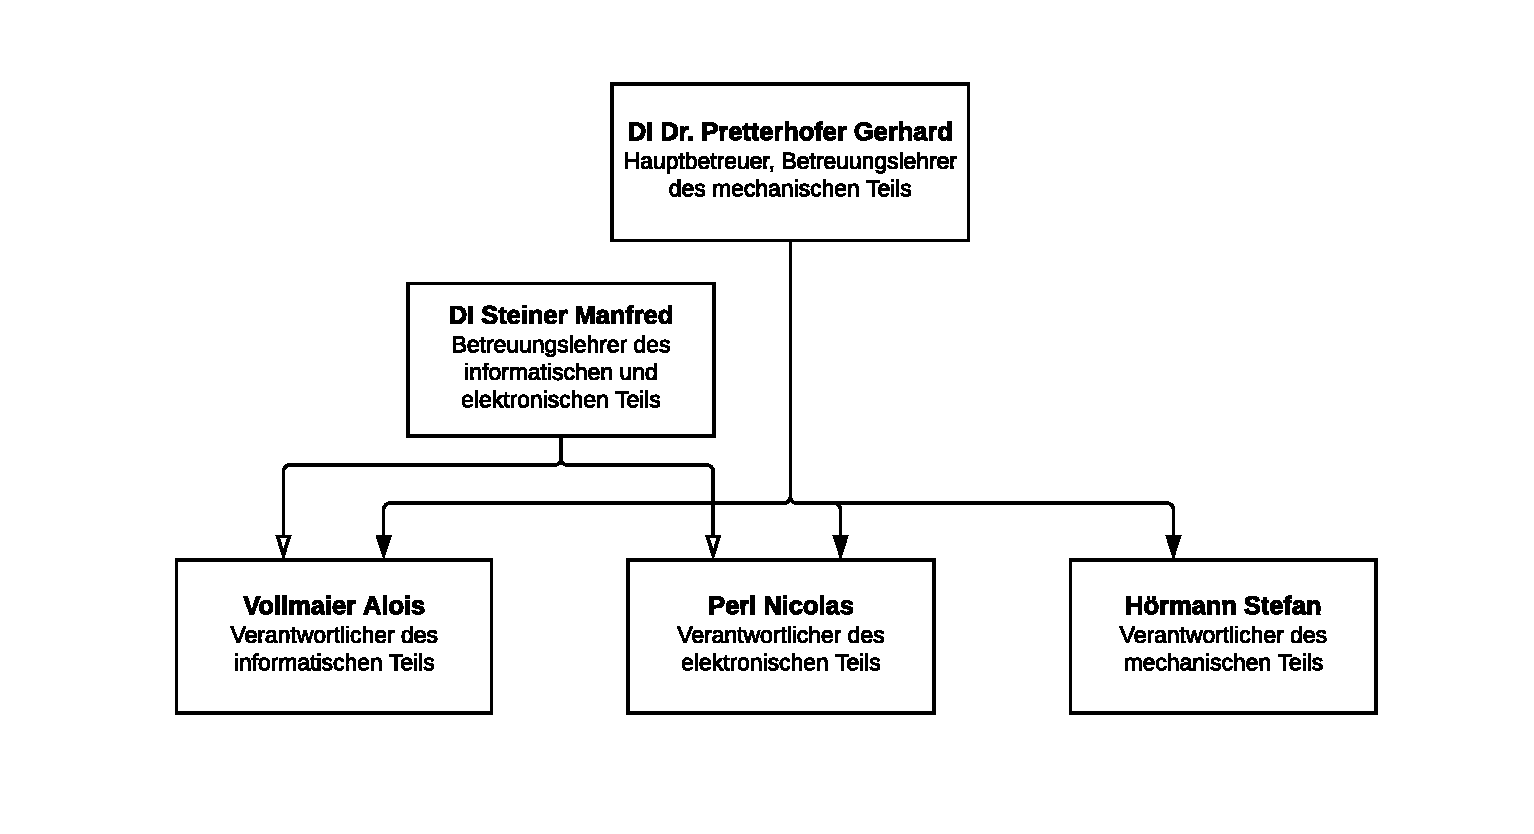
\includegraphics[width=0.80\textwidth]{fig/Hierachie_Reshuffled.pdf}
    \caption{Betreuerübersicht}
    \label{Bild über ganze Seitenbreite}
\end{figure}


\section{Konzept}
Wir setzten uns als Ziel eine Maschine zu entwickeln, welche das Mischen, sowie das Ausgeben von Spielkarten übernimmt.
Die Idee ist es, diese Verfahren möglichst platzsparend, zeiteffizient und detailliert durchdacht und optimiert zu realisieren.\\

\begin{wrapfigure}{r}{0.34\textwidth}
    \vspace{-40pt}
    \begin{center}
        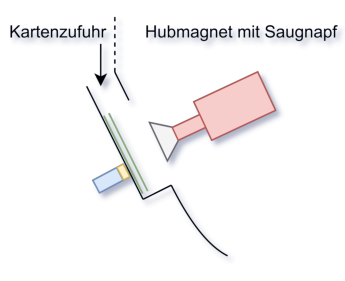
\includegraphics[width=0.35\textwidth]{fig/Reshuffled_Version_3_prinzip}
    \end{center}
    \caption{Kartenentnahme}
    \label{Kartenentnahme}
    \vspace{-15pt}
\end{wrapfigure}

Grundsätzlich basiert das Mischprinzip auf einer Art "Fächersystem".
Eingelegte Karten gelangen mithilfe eines ausgeklügelten Systems, welches aus einem Hubmagneten mit integriertem Saugnapf besteht, aus dem Einlegefach.
Erfolgt die Kartenentnahme, rutscht die Karte in ein zufälliges Fach des Lagerrads. Anschließend wird dieses Lagerrad in Drehbewegung versetzt um die gelagerten Karten auszugeben.

Der Benutzer steuert diese Maschiene auf einer GUI welche auf einem 7" LCD Display angezeigt wird. Systemintern steuert ein 8Bit Mikrocontroller der AVR-Familie den Ablauf.

%============================================
\chapter{Mechanik}
\lohead{Stefan Hörmann}
\label{sec:Mechanik}
\section{Beschreibung}

Der mechanische Teil begann mit dem Variantenvergleich. Dabei wurden verschiedene Varianten der Maschine basierend auf deren Kosten, deren Schnelligkeit und deren Realisierbarkeit verglichen.
Hier muss zusätzlich darauf geachtet werden, dass die benötigten Bauteile weitestgehend in der Lehranstalt oder privat gefertigt werden können.\\

\begin{wrapfigure}{r}{0.5\textwidth}
    \vspace{-50pt}
    \begin{center}
        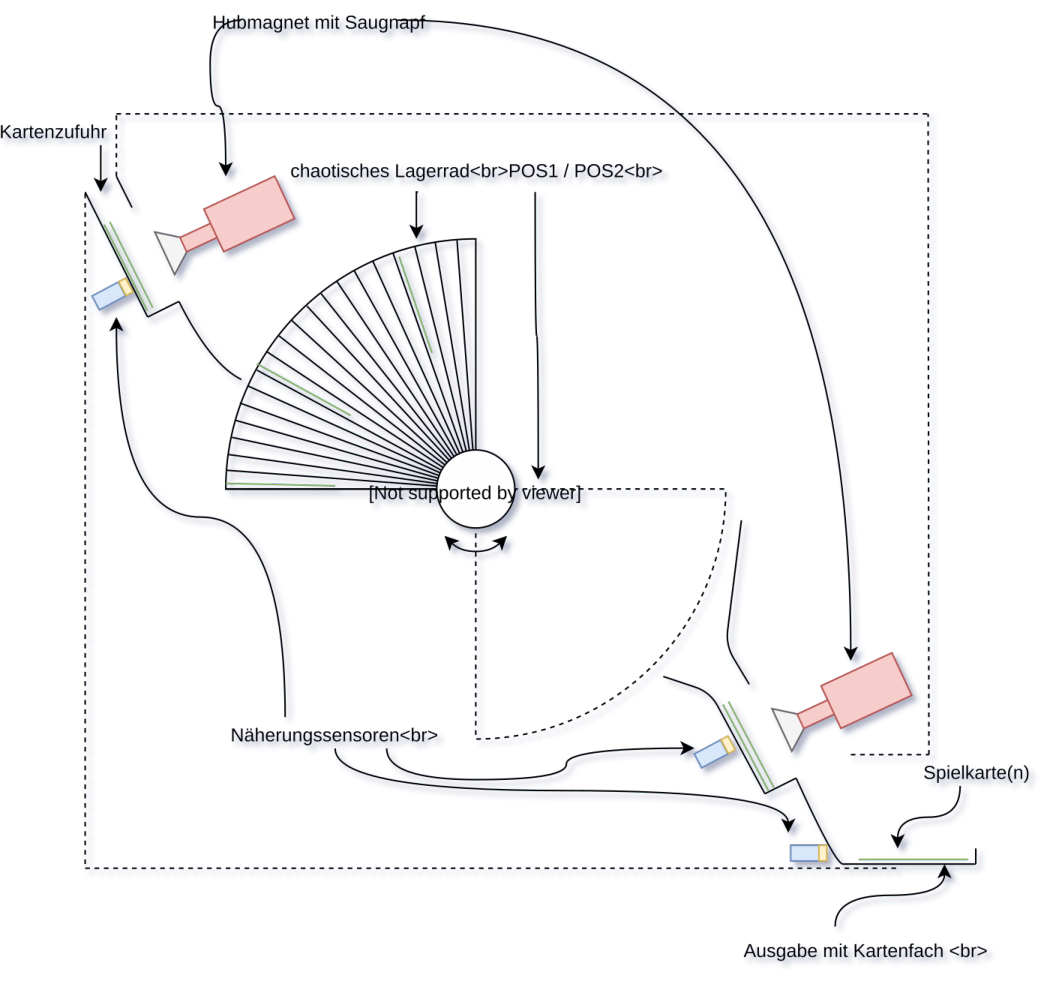
\includegraphics[width=0.5\textwidth]{fig/Reshuffled_Version_3_0_prinzip}
    \end{center}
    \caption{Variantenvergleich Version 3}
    \label{Variantenvergleich}
    \vspace{-15pt}
\end{wrapfigure}

Danach wurde der Motor ausgewählt. Dies erfolgte über diverse Berechnungen, welche die einwirkenden Kräfte auf das Lagerrad sowie dei benötigten Beschleunigungskräfte berücksichtigten.
Als solches erledigt wurde, ist der Hubmagnet ausgewählt worden. Dabei wurde auf die Bauform, auf die Art des Aufbaus und den Preis geachtet.
\\\\
Die CAD-Zeichnungen des Lagerrads sollten vor den Ferien fertiggestellt werden und für die Werkstatt freigegeben werden, sodass diese noch vor den Ferien für Testdurchläufe des Motors zur Verfügung stehen.
Die 3D-Druck Teile sollten vor den Ferien ebenfalls fertig gedruckt sein.
\\\\
Der größte Teil der Arbeit besteht in der Konstruktion der gesamten Maschine, da die Teile hauptsächlich 3D-gedruckt werden, muss darauf geachtet werden, dass alle Teile so konstruiert werden, dass dies ohne Probleme funktioniert.
Für die CAD-Konstruktion wird das bereits in der Schule gelernte Programm Inventor benutzt. Alle im Nachhinein benötigten Belastungsanalysen sowie Simulationen werden mit diesem Programm erledigt.


%============================================
\chapter{Elektronik}
\lohead{Nicolas Perl}
\label{sec:Elektronik}
\section{Beschreibung}

Der elektrische Teil dieser Diplomarbeit umfasst das Designen eines Schaltplans einer Platine, das darauffolgende Layouten sowie dem Bestücken der Platine. Darauf folgen Tests und Verbesserungen.\\

Die Platine, gesteuert vom Mikroprozessor Atmega324P, hat die Aufgabe 3 kapazitive Sensoren einzulesen, 2 Hubmagneten anzusteuern und eine Schrittmotorsteuerung anzusteuern.
Zusätzlich soll der Mikroprozessor im Stande dazu sein, Befehle vom Raspberry Pi 3B+ über UART zu erhalten. Debugging über eine zweite UART - Schnitte via Mini USB soll ebenfalls möglich sein. \\

Ein weiterer großer Teil der Elektronik besteht aus der Spannungsversorgung. Über eine Steuerspannung von 12V, welche wir über ein Notebook-Netzteil bekommen, ist die gesamte Hardware zu versorgen.
Die 12V Steuerspannung dient zur Versorgung vom Schrittmotor, von den 3 kapazitiven Sensoren und von den 2 Hubmagneten. Über einen DC/DC Wandler sollen 5V erzeugt und mit diesen der Raspberry Pi versorgt werden.
Über den 3.3V Ausgang des RPI wird folgend der Atmega324P versorgt.





%============================================
\chapter{Informatik}
\lohead{Alois Vollmaier}
\label{sec:Informatik}
\section{Beschreibung}

Den informatischen Teil der Arbeit kann man grundsätzlich in 2 Bereiche aufteilen. Es soll eine einfache grafische Benutzeroberfläche gestaltet werden, auf welcher man den Mischvorgang steuern sowie grundlegende Einstellungen des Spieles vornehmen kann.
Aus programmtechnischen Gründen wird hierfür die Programmiersprache Java und das GUI-Toolkit Swing verwendet. \\
Die Hardwarekomponenten setzen sich aus einem Raspberry Pi 3B+ und einem 7" LCD Touchscreen der Firma Elecrow zusammen. \\

Zusätzlich besteht dieser Teilbereich der Arbeit auch aus der hardwarenahen Programmierung der Hauptplatine. Mithilfe der Programmiersprache C sollte der verbaute 8-Bit Mikrocontroller der AVR-Familie namens ATmega324P programmiert werden.
Dieser steuert den gesamten Ablauf der Maschiene. \\

Der Datenaustausch zwischen der Hauptplatine und dem Raspberry PI erfolgt über die serielle Schnittstelle namens UART.
Im Hintergrund wird gleichzeitig eine Json Logdatei
%============================================
\chapter{Projektplanung}
\lohead{ReShuffled Projektplanung}
\label{sec:Projektplanung}
\section{Meilensteine}
\begin{table}[h!]
    \begin{tabular}{ll}
        \hline
        \rowcolor[HTML]{C0C0C0}
        \multicolumn{2}{c}{\cellcolor[HTML]{C0C0C0}\textbf{Meilensteine}}                      \\ \hline
        \rowcolor[HTML]{EFEFEF}
        \multicolumn{1}{l|}{\cellcolor[HTML]{EFEFEF}Datum} & Beschreibung                      \\ \hline
        \multicolumn{1}{l|}{15. Mai 2019}                   & Vollenden des Variantenvergleichs \\ \hline
        \multicolumn{1}{l|}{01. Aug.2019}                    & Fertigstellung der CAD Zeichnung  \\ \hline
        \multicolumn{1}{l|}{15. Sep. 2019}                   & Fertigstellung der Hardware       \\ \hline
        \multicolumn{1}{l|}{31. Okt. 2019}                   & Abschließen des Testaufbaus       \\ \hline
        \multicolumn{1}{l|}{01. Dez. 2019}                    & Fertigstellung der Software       \\ \hline
    \end{tabular}
\end{table}

\section{Aufgabenplanung bis September}

Ziele des Herrn Hörmann:
\begin{itemize}
    \item Standartmäßig ist ein schwarzer Punkt davor.
    \item Die Länge ist nicht von Bedeutung, Zeilen werden automatisch umgebrochen.
\end{itemize}

\noindent\hrulefill

Ziele des Herrn Pearl:
\begin{itemize}
    \item Standartmäßig ist ein schwarzer Punkt davor.
    \item Die Länge ist nicht von Bedeutung, Zeilen werden automatisch umgebrochen.
\end{itemize}

\noindent\hrulefill

Ziele des Herrn Vollmaier:
\begin{itemize}
    \item Standartmäßig ist ein schwarzer Punkt davor.
    \item Die Länge ist nicht von Bedeutung, Zeilen werden automatisch umgebrochen.
\end{itemize}

%============================================
\chapter{Anhang}




